% Options for packages loaded elsewhere
\PassOptionsToPackage{unicode}{hyperref}
\PassOptionsToPackage{hyphens}{url}
%
\documentclass[
]{article}
\usepackage{amsmath,amssymb}
\usepackage{lmodern}
\usepackage{iftex}
\ifPDFTeX
  \usepackage[T1]{fontenc}
  \usepackage[utf8]{inputenc}
  \usepackage{textcomp} % provide euro and other symbols
\else % if luatex or xetex
  \usepackage{unicode-math}
  \defaultfontfeatures{Scale=MatchLowercase}
  \defaultfontfeatures[\rmfamily]{Ligatures=TeX,Scale=1}
\fi
% Use upquote if available, for straight quotes in verbatim environments
\IfFileExists{upquote.sty}{\usepackage{upquote}}{}
\IfFileExists{microtype.sty}{% use microtype if available
  \usepackage[]{microtype}
  \UseMicrotypeSet[protrusion]{basicmath} % disable protrusion for tt fonts
}{}
\makeatletter
\@ifundefined{KOMAClassName}{% if non-KOMA class
  \IfFileExists{parskip.sty}{%
    \usepackage{parskip}
  }{% else
    \setlength{\parindent}{0pt}
    \setlength{\parskip}{6pt plus 2pt minus 1pt}}
}{% if KOMA class
  \KOMAoptions{parskip=half}}
\makeatother
\usepackage{xcolor}
\IfFileExists{xurl.sty}{\usepackage{xurl}}{} % add URL line breaks if available
\IfFileExists{bookmark.sty}{\usepackage{bookmark}}{\usepackage{hyperref}}
\hypersetup{
  hidelinks,
  pdfcreator={LaTeX via pandoc}}
\urlstyle{same} % disable monospaced font for URLs
\usepackage[margin=1in]{geometry}
\usepackage{longtable,booktabs,array}
\usepackage{calc} % for calculating minipage widths
% Correct order of tables after \paragraph or \subparagraph
\usepackage{etoolbox}
\makeatletter
\patchcmd\longtable{\par}{\if@noskipsec\mbox{}\fi\par}{}{}
\makeatother
% Allow footnotes in longtable head/foot
\IfFileExists{footnotehyper.sty}{\usepackage{footnotehyper}}{\usepackage{footnote}}
\makesavenoteenv{longtable}
\usepackage{graphicx}
\makeatletter
\def\maxwidth{\ifdim\Gin@nat@width>\linewidth\linewidth\else\Gin@nat@width\fi}
\def\maxheight{\ifdim\Gin@nat@height>\textheight\textheight\else\Gin@nat@height\fi}
\makeatother
% Scale images if necessary, so that they will not overflow the page
% margins by default, and it is still possible to overwrite the defaults
% using explicit options in \includegraphics[width, height, ...]{}
\setkeys{Gin}{width=\maxwidth,height=\maxheight,keepaspectratio}
% Set default figure placement to htbp
\makeatletter
\def\fps@figure{htbp}
\makeatother
\setlength{\emergencystretch}{3em} % prevent overfull lines
\providecommand{\tightlist}{%
  \setlength{\itemsep}{0pt}\setlength{\parskip}{0pt}}
\setcounter{secnumdepth}{-\maxdimen} % remove section numbering
\usepackage{booktabs}
\usepackage{longtable}
\usepackage{array}
\usepackage{multirow}
\usepackage{wrapfig}
\usepackage{float}
\usepackage{colortbl}
\usepackage{pdflscape}
\usepackage{tabu}
\usepackage{threeparttable}
\usepackage{threeparttablex}
\usepackage[normalem]{ulem}
\usepackage{makecell}
\usepackage{xcolor}
\ifLuaTeX
  \usepackage{selnolig}  % disable illegal ligatures
\fi

\author{}
\date{\vspace{-2.5em}}

\begin{document}

\hypertarget{risk-summary-federal-funding}{%
\section{Risk Summary: Federal
Funding}\label{risk-summary-federal-funding}}

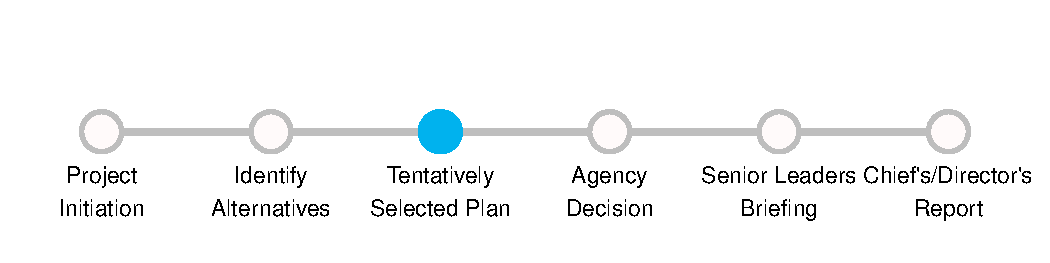
\includegraphics{RiskItemReport_files/figure-latex/milestoneplot-1.pdf}

\hypertarget{lead-discipline-project-management}{%
\subsubsection{Lead Discipline: Project
Management}\label{lead-discipline-project-management}}

\hypertarget{there-will-be-a-gap-in-federal-funding-streams-for-the-study-after-the-amm.-nfs-can-accelerate-their-share-of-the-funding.-three-various-efforts-are-in-play-during-the-spring-earmark-workplan-infrastructure-bill-which-could-help-in-getting-needed-federal-funding.}{%
\paragraph{There will be a gap in Federal funding streams for the study
after the AMM. NFS can accelerate their share of the funding. Three
various efforts are in play during the spring (earmark, workplan,
infrastructure bill) which could help in getting needed Federal
funding.}\label{there-will-be-a-gap-in-federal-funding-streams-for-the-study-after-the-amm.-nfs-can-accelerate-their-share-of-the-funding.-three-various-efforts-are-in-play-during-the-spring-earmark-workplan-infrastructure-bill-which-could-help-in-getting-needed-federal-funding.}}

15-FEB-22: Funding from IIJA was approved in early 2022 to fully fund
the Federal portion of the study at \$3M. Based on the \$4.5M study
budget, these federal funds will be sufficient to fund the study through
the TSP (Spring 2023)

\hypertarget{event-likelihood-very-unlikely-5-to-30}{%
\subsection{Event Likelihood: Very Unlikely (5\% to
30\%)}\label{event-likelihood-very-unlikely-5-to-30}}

There are several avenues in play, subject to change

\begin{longtable}[]{@{}
  >{\raggedright\arraybackslash}p{(\columnwidth - 4\tabcolsep) * \real{0.2781}}
  >{\raggedright\arraybackslash}p{(\columnwidth - 4\tabcolsep) * \real{0.3195}}
  >{\raggedright\arraybackslash}p{(\columnwidth - 4\tabcolsep) * \real{0.4024}}@{}}
\toprule
\begin{minipage}[b]{\linewidth}\raggedright
Cost Impact
\end{minipage} & \begin{minipage}[b]{\linewidth}\raggedright
Schedule Impact
\end{minipage} & \begin{minipage}[b]{\linewidth}\raggedright
Performance Impact
\end{minipage} \\
\midrule
\endhead
\emph{Lowest} \$0 & \emph{Lowest} 0 days & \textbf{\emph{Performance
Impact:}} Team would need to stop work if all funds exhausted. \\
1-APR-2022: There is sufficient time to plan ahead to maintain funding
streams consistent with the authorized budget. The rating was downgraded
from ``major problem'' to ``minor problem'', but is dependent upon
receiving a decision to the exception request by 1-JUL to avoid schedule
impacts. & & \\
\emph{Highest} \$0 & \emph{Highest} 0 days & \textbf{\emph{Performance
Impact Type:}} Agency Strategy \\
NA & There is a risk that if there is a gap in Federal funding for too
long, NFS accelerated funds may be exhausted, causing a study delay and
risk to 3-year schedule & Team would need to stop work if all funds
exhausted. \\
1-APR-2022: There is sufficient time to plan ahead to maintain funding
streams consistent with the authorized budget. The rating was downgraded
from ``major problem'' to ``minor problem'', but is dependent upon
receiving a decision to the exception request by 1-JUL to avoid schedule
impacts. & & \\
\bottomrule
\end{longtable}

\hypertarget{risk-treatments}{%
\subsection{Risk Treatments}\label{risk-treatments}}

\begin{verbatim}
## Warning in add_header_above(., c(Measures = 2, Impacts = 2, Implemented = 1)):
## Please specify format in kable. kableExtra can customize either HTML or LaTeX
## outputs. See https://haozhu233.github.io/kableExtra/ for details.
\end{verbatim}

\begin{verbatim}
## Warning in kable_styling(.): Please specify format in kable. kableExtra can
## customize either HTML or LaTeX outputs. See
## https://haozhu233.github.io/kableExtra/ for details.
\end{verbatim}

\begin{longtable}[]{@{}rlrrl@{}}
\toprule
\endhead
1 & Sponsor will accelerate their share in the full amount & 0 & 0 &

\includegraphics{C:/workspace/e-rarr/images/check.png} \\
2 & PM is working on all three avenues to obtain Federal funds (earmark,
workplan, infrastructure bill) & 0 & 0 &

\includegraphics{C:/workspace/e-rarr/images/check.png} \\
3 & Team will develop forecast of when funds would be exhausted and will
elevate to management to track closely & 0 & 0 &

\includegraphics{C:/workspace/e-rarr/images/check.png} \\
\bottomrule
\end{longtable}

\#\#test

\end{document}
